\documentclass[11pt]{article}
\usepackage[margin=1in]{geometry}
\usepackage{graphicx}
\usepackage{enumitem}
\usepackage{parskip}

\title{Instructor Onboarding}
\author{}
\date{}

\begin{document}

\maketitle

\section*{Current Status}
Verified on March 16, 2026 against the live Supabase-backed portal.

Verified instructor workflows:
\begin{itemize}
  \item login and route protection
  \item dashboard load
  \item attendance update
  \item student instructional note creation
  \item session instructional note creation
  \item instructor follow-up flag creation
  \item direct access to \texttt{/families} and \texttt{/messaging} correctly redirected back to \texttt{/dashboard}
\end{itemize}

\section*{What Instructor Is For}
Instructor is the narrow teaching role.

Instructor owns:
\begin{itemize}
  \item attendance for assigned sessions
  \item instructional context for assigned students
  \item read-only trend review
\end{itemize}

Instructor does not own:
\begin{itemize}
  \item family messaging
  \item billing
  \item settings
  \item resource publishing
  \item score entry
  \item staffing or schedule edits
\end{itemize}

\section*{Core Boundaries}
Instructor can:
\begin{itemize}
  \item access \texttt{dashboard}, \texttt{calendar}, \texttt{cohorts}, \texttt{attendance}, and \texttt{academics}
  \item update attendance for assigned sessions
  \item update tasks assigned to them
  \item create student instructional notes
  \item create session instructional notes
  \item create follow-up flags for a student or session
  \item read classroom accommodations
  \item review teaching context for assigned students
\end{itemize}

Instructor cannot:
\begin{itemize}
  \item open \texttt{students}, \texttt{families}, \texttt{messaging}, \texttt{billing}, \texttt{integrations}, \texttt{programs}, or \texttt{settings}
  \item view guardian contact detail pages
  \item change schedules or staffing
  \item use TA checklist or coverage tools
\end{itemize}

\section*{Screens}
\subsection*{Instructor Dashboard}
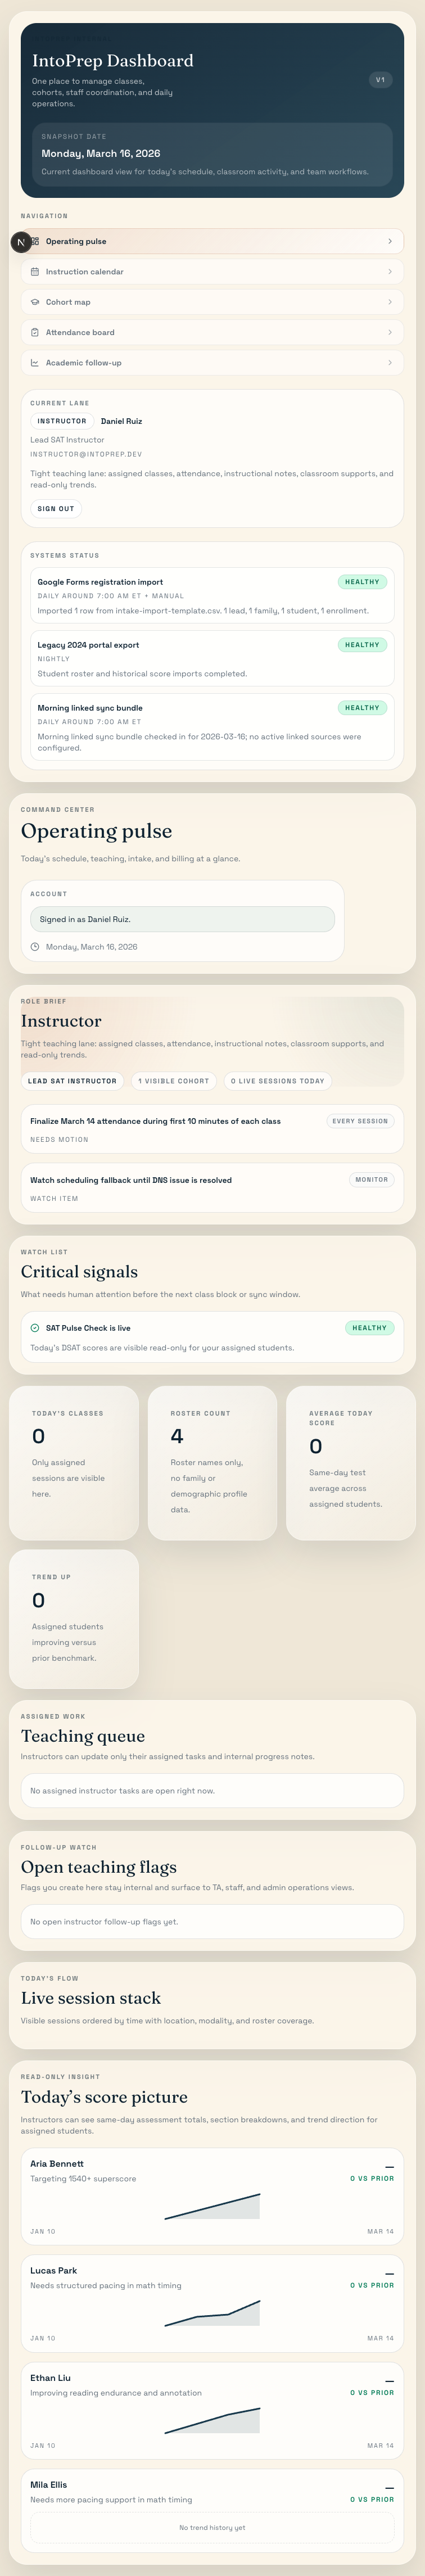
\includegraphics[width=\textwidth]{assets/instructor-dashboard.png}

\subsection*{Instructor Attendance}
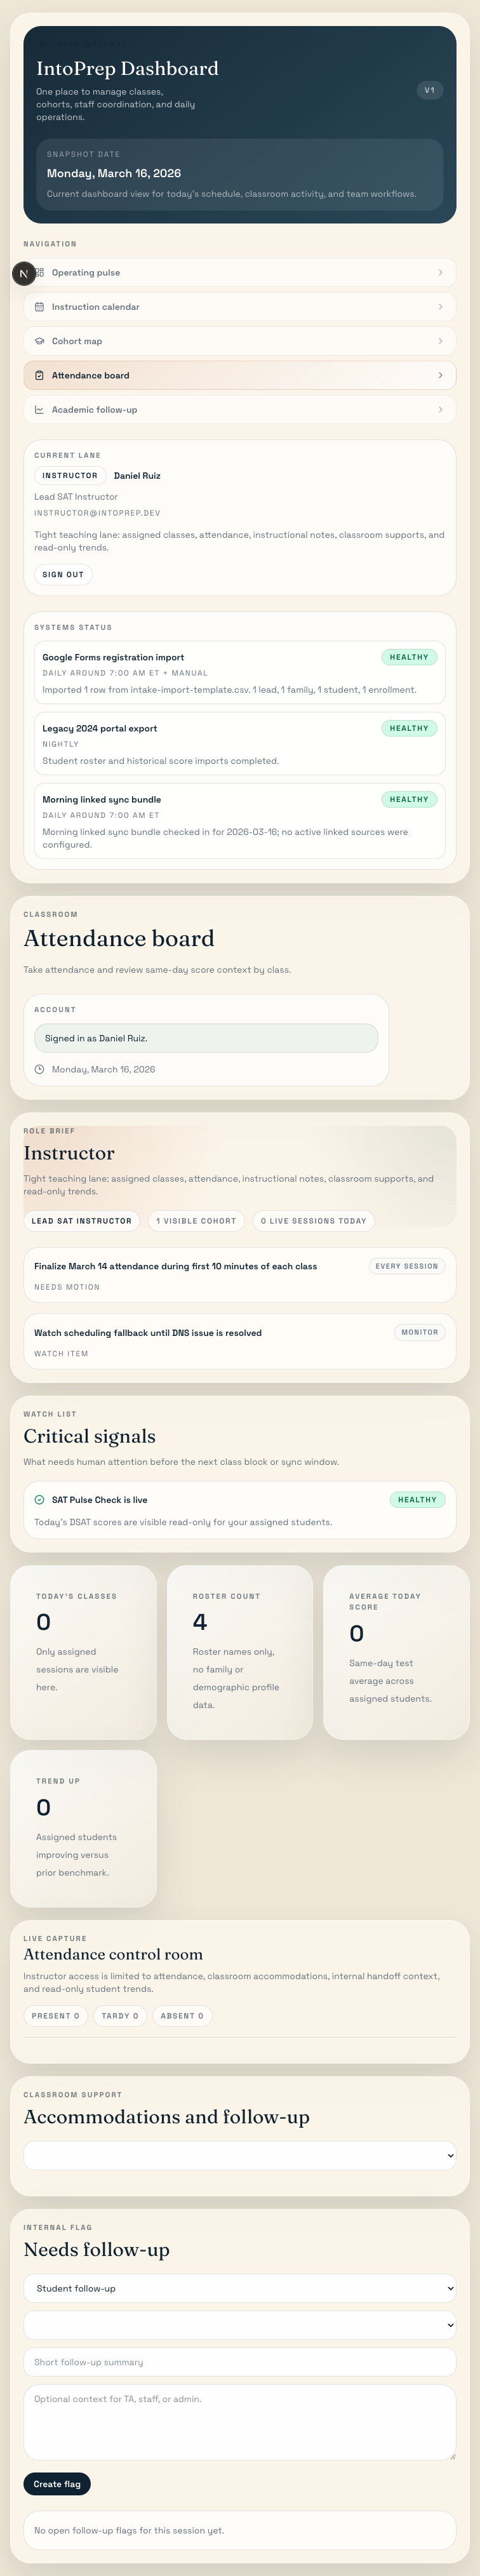
\includegraphics[width=\textwidth]{assets/instructor-attendance.png}

\subsection*{Instructor Academics}
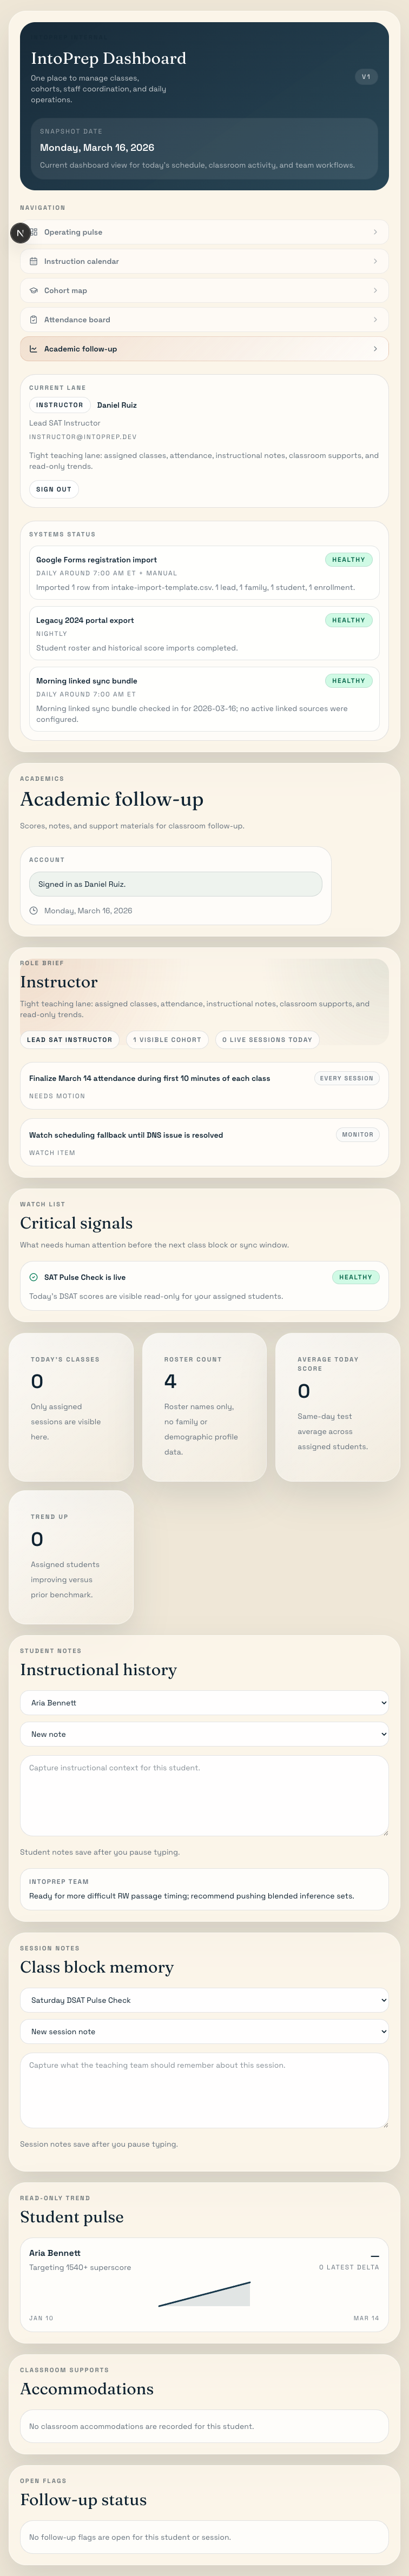
\includegraphics[width=\textwidth]{assets/instructor-academics.png}

\section*{First Login Walkthrough}
\begin{enumerate}
  \item Sign in at \texttt{/login}.
  \item Start on ``Operating pulse''.
  \item Review:
  \begin{itemize}
    \item assigned sessions
    \item assigned tasks
    \item trend snippets for assigned students
  \end{itemize}
  \item Open ``Attendance board''.
  \item Open ``Academic follow-up''.
\end{enumerate}

\section*{Daily Workflow}
\subsection*{1. Start On The Dashboard}
Use the dashboard to confirm:
\begin{itemize}
  \item today’s teaching blocks
  \item current assigned work
  \item high-level trend context
\end{itemize}

\subsection*{2. Update Attendance}
Open ``Attendance board'' for your assigned session.
\begin{itemize}
  \item mark attendance
  \item review teaching context on the current roster
  \item confirm the session is ready from the instructor side
\end{itemize}

Smoke test verification:
\begin{itemize}
  \item instructor attendance update succeeded on ``session-sat-mock''
\end{itemize}

\subsection*{3. Add Student Instructional Notes}
Open ``Academic follow-up''.
\begin{itemize}
  \item document student-specific instructional context
  \item keep the note operational and classroom-focused
\end{itemize}

Smoke test verification:
\begin{itemize}
  \item instructor student note creation succeeded
\end{itemize}

\subsection*{4. Add Session Instruction Notes}
Use the session note area in ``Academic follow-up'' to capture what the teaching team should remember about a specific class block.
\begin{itemize}
  \item select the session
  \item enter a concise internal note
  \item let the autosave complete
\end{itemize}

Smoke test verification:
\begin{itemize}
  \item instructor session note save succeeded
\end{itemize}

\subsection*{5. Create A Follow-Up Flag}
Open ``Attendance board'' and use the ``Needs follow-up'' area.
\begin{itemize}
  \item choose whether the flag is for a student or the session
  \item add a short summary
  \item add optional context for TA, staff, or admin
  \item submit the flag
\end{itemize}

Smoke test verification:
\begin{itemize}
  \item instructor follow-up flag save succeeded
  \item the new flag appeared in the TA dashboard follow-up watch
\end{itemize}

\section*{Complete Capability Map}
Instructor is the tightest teaching role in the portal.

Use instructor for:
\begin{itemize}
  \item attendance
  \item assigned tasks
  \item student instructional notes
  \item session instructional notes
  \item read-only trends
  \item read-only classroom accommodations
  \item lightweight internal follow-up flags
\end{itemize}

Do not use instructor for:
\begin{itemize}
  \item family communication
  \item billing
  \item score entry
  \item resource publishing
  \item staffing or schedule changes
  \item checklist, coverage, or TA support tooling
\end{itemize}

\section*{How To Work Assigned Tasks}
\begin{enumerate}
  \item Review the teaching queue from the dashboard.
  \item Open the assigned item.
  \item Update status and progress notes as work moves.
  \item Keep notes short and instructional, not administrative.
\end{enumerate}

\section*{How To Use Read-Only Accommodations}
\begin{enumerate}
  \item Open ``Attendance board'' or ``Academic follow-up''.
  \item Review the accommodation badges or support notes for the current student.
  \item Use those supports in the classroom.
  \item Do not try to edit accommodation content from the instructor role.
\end{enumerate}

\section*{How To Use Trend Review}
\begin{enumerate}
  \item Open ``Academic follow-up''.
  \item Select the student.
  \item Review the latest score picture and trend direction.
  \item Use that context to guide teaching, but do not enter or change scores from this role.
\end{enumerate}

\section*{How To Use Calendar And Cohort Views}
\begin{itemize}
  \item calendar:
  use it to confirm when and where your assigned sessions are happening.
  \item cohorts:
  use it to review the teaching group context for assigned classes.
  \item both views are read-only from the instructor role.
\end{itemize}

\section*{Guardrails}
\begin{itemize}
  \item no family pages
  \item no messaging pages
  \item no billing pages
  \item no schedule edits
  \item no checklist or coverage tools
\end{itemize}

\section*{Verified Behavior}
Verified in the live browser pass:
\begin{itemize}
  \item instructor login succeeded
  \item dashboard, attendance, and academics loaded
  \item attendance update succeeded through the live API
  \item student note save succeeded through the live API
  \item session note save succeeded through the live API
  \item instructor follow-up flag save succeeded through the live API
  \item direct access to \texttt{/families} redirected back to \texttt{/dashboard}
  \item direct access to \texttt{/messaging} redirected back to \texttt{/dashboard}
\end{itemize}

\section*{Recommended First-Day Checklist}
\begin{itemize}
  \item review dashboard and current sessions
  \item update attendance on one assigned session
  \item add one student instructional note on an assigned student
  \item add one session note on an assigned session
  \item create one follow-up flag on an assigned student or session
\end{itemize}

\end{document}
\ No newline at end of file
